% Created 2017-02-22 Wed 13:57
\documentclass[t,10pt]{beamer}
\usepackage[utf8]{inputenc}
\usepackage[T1]{fontenc}
\usepackage{fixltx2e}
\usepackage{graphicx}
\usepackage{grffile}
\usepackage{longtable}
\usepackage{wrapfig}
\usepackage{rotating}
\usepackage[normalem]{ulem}
\usepackage{amsmath}
\usepackage{textcomp}
\usepackage{amssymb}
\usepackage{capt-of}
\usepackage{hyperref}
\usepackage{color}
\usepackage{listings}
\mode<beamer>{\usetheme{Madrid}}
\lstset{
language=sh,
otherkeywords={=, +, [, ], (, ), \{, \}, *, $},
emph={addgroup,adduser,alias,ant,apropos,apt-get,aptitude,aspell,awk,basename,bash,bc,bg,break,builtin,bzip2,cal,case,cat,cd,cfdisk,chgrp,chkconfig,chmod,chown,chroot,cksum,clear,cmp,comm,command,continue,cp,cron,crontab,csplit,cut,date,dc,dd,ddrescue,declare,df,diff,diff3,    dig,dir,dircolors,dirname,dirs,dmesg,du,echo,egrep,eject,enable,env,    ethtool,eval,exec,exit,expand,expect,export,expr,false,fdformat,    fdisk,fg,fgrep,file,find,fmt,fold,for,format,free,fsck,ftp,function,    fuser,gawk,getopts,    git,    grep,groups,gzip,    gunzip,    ,hash,head,help,history,hostname,    id,if,ifconfig,ifdown,ifup,import,install,    java, java6, java_cur    join,kill,killall,    let,ln,local,locate,logname,logout,look,lpc,lpr,lprint,lprintd,    lprintq,lprm,ls,lsof,make,man,mkdir,mkfifo,mkisofs,mknod,mmv,more,    mount,mtools,mtr,mv,    mysql,    netstat,nice,nl,nohup,notify-send,    noweb,noweave,    nslookup,op,    open,passwd,paste,pathchk,ping,pkill,popd,pr,printcap,printenv,    printf,ps,pushd,pwd,quota,quotacheck,quotactl,ram,rcp,read,    readarray,readonly,reboot,remsync,rename,renice,return,rev,rm,rmdir,    rsync,scp,screen,sdiff,sed,select,seq,set,sftp,shift,shopt,shutdown,    sleep,slocate,sort,source,split,ssh,strace,su,sudo,sum,    svn, svn2git,    symlink,sync,    tail,tar,tee,test,time,times,top,touch,tr,traceroute,trap,true,    tsort,tty,type,ulimit,umask,umount,unalias,uname,unexpand,uniq,    units,    unrar,    unset,unshar,until,useradd,usermod,users,uudecode,uuencode,    vdir,vi,vmstat,watch,wc,Wget,whereis,which,while,who,whoami,write,    zcat},
breaklines=true,
keywordstyle=\color{blue},
stringstyle=\color{red},
emphstyle=\color{black}\bfseries,
commentstyle=\color{gray}\slshape
}
\hypersetup{colorlinks=true, linkcolor=blue}
\AtBeginSection[]{\begin{frame}<beamer>\frametitle{Topic}\tableofcontents[currentsection]\end{frame}}
\lstset{basicstyle=\scriptsize\ttfamily}
\usetheme{Madrid}
\author{Stephen A. Sefick}
\date{2017-02-23}
\title{Advanced Shell Scripting for Bioinformatics}
\titlegraphic{
\includegraphics[width=\textwidth,height=.3\textheight]{figures/GNU_DNA_TUX.png}}\vspace{0.25in}
\hypersetup{
 pdfauthor={Stephen A. Sefick},
 pdftitle={Advanced Shell Scripting for Bioinformatics},
 pdfkeywords={},
 pdfsubject={},
 pdfcreator={Emacs 24.5.1 (Org mode 8.3.6)}, 
 pdflang={English}}
\begin{document}

\maketitle
\begin{frame}{Outline}
\tableofcontents
\end{frame}



\section{Introduction}
\label{sec:orgheadline16}
\begin{frame}[label={sec:orgheadline1}]{Motivation: why write a bash script?}
\end{frame}
\begin{frame}[label={sec:orgheadline2}]{Motivation: why write a bash script?}
\begin{enumerate}[<+->]
\item Reusable 
\begin{itemize}
\item Do something once; do it a thousand times \vspace{0.25in}
\end{itemize}
\item Remember what you did
\begin{itemize}
\item analysis documentation
\item reproducible research
\item literate programming \vspace{0.25in}
\end{itemize}
\item Deploy-able on desktop or supercomputer \vspace{0.25in}
\item Computer Programming is JUST DARN FUN!!!
\end{enumerate}
\end{frame}

\begin{frame}[label={sec:orgheadline3}]{Basic Bash Scripting}
\end{frame}
\begin{frame}[label={sec:orgheadline4}]{Basic Bash Scripting}
\begin{enumerate}[<+->]
\item What is a script?
\begin{itemize}
\item a "recipe" for the computer \vspace{0.25in}
\end{itemize}
\item A collection of instructions in an \alert{interpreted language}
\begin{itemize}
\item Bash, R, Python, Perl, etc.
\item Instructions executed at run-time
\item with language specified in the shebang line \vspace{0.25in}
\end{itemize}
\item Human-readable (next step literate programming)
\begin{itemize}
\item comment, comment, comment!!!
\item worst enemy in 6 months?
\item YOU ARE!!!! \vspace{0.25in}
\end{itemize}
\end{enumerate}
\end{frame}
\begin{frame}[label={sec:orgheadline5}]{Anatomy of a script}
\end{frame}
\begin{frame}[label={sec:orgheadline6}]{Anatomy of a script}
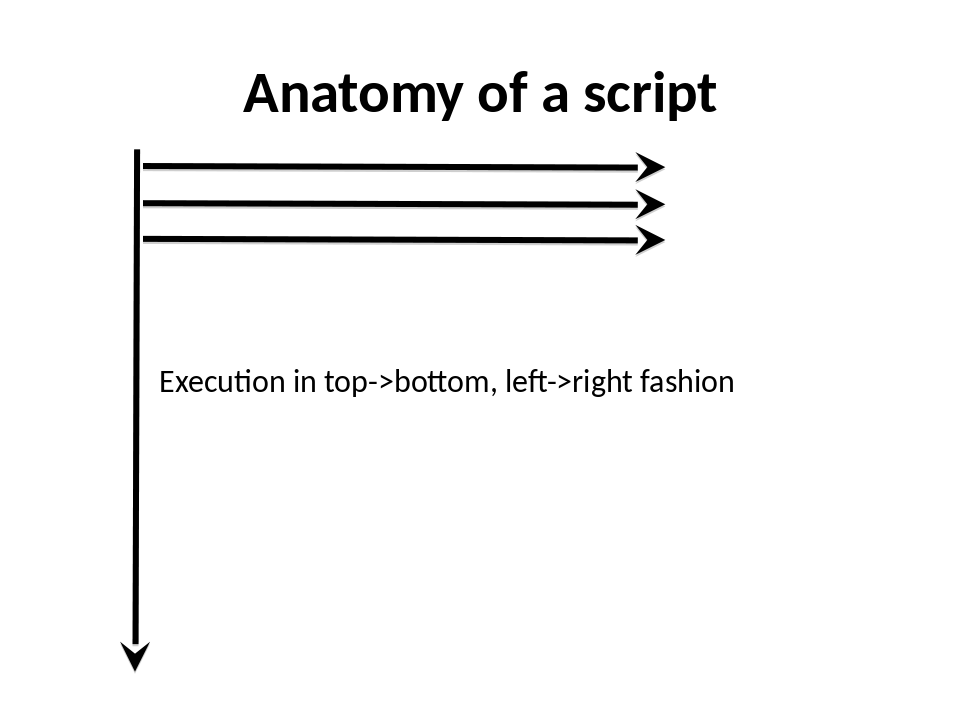
\includegraphics[width=.9\linewidth]{figures/1_anatomy_shell_script.png}
\end{frame}
\begin{frame}[label={sec:orgheadline7}]{Anatomy of a script}
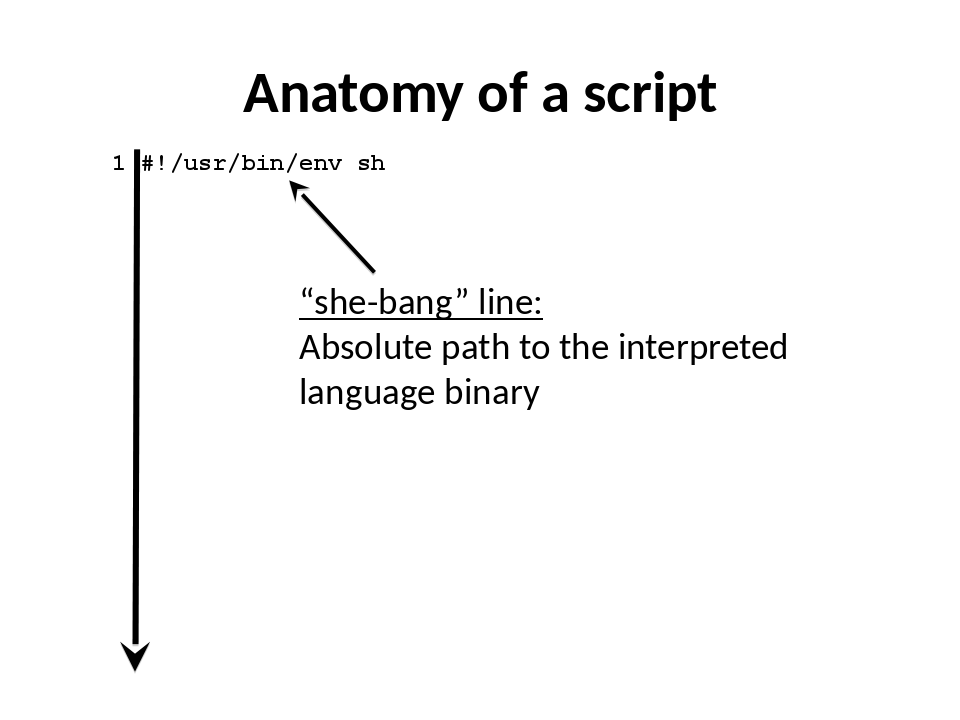
\includegraphics[width=.9\linewidth]{figures/2_anatomy_shell_script.png}
\end{frame}
\begin{frame}[label={sec:orgheadline8}]{Anatomy of a script}
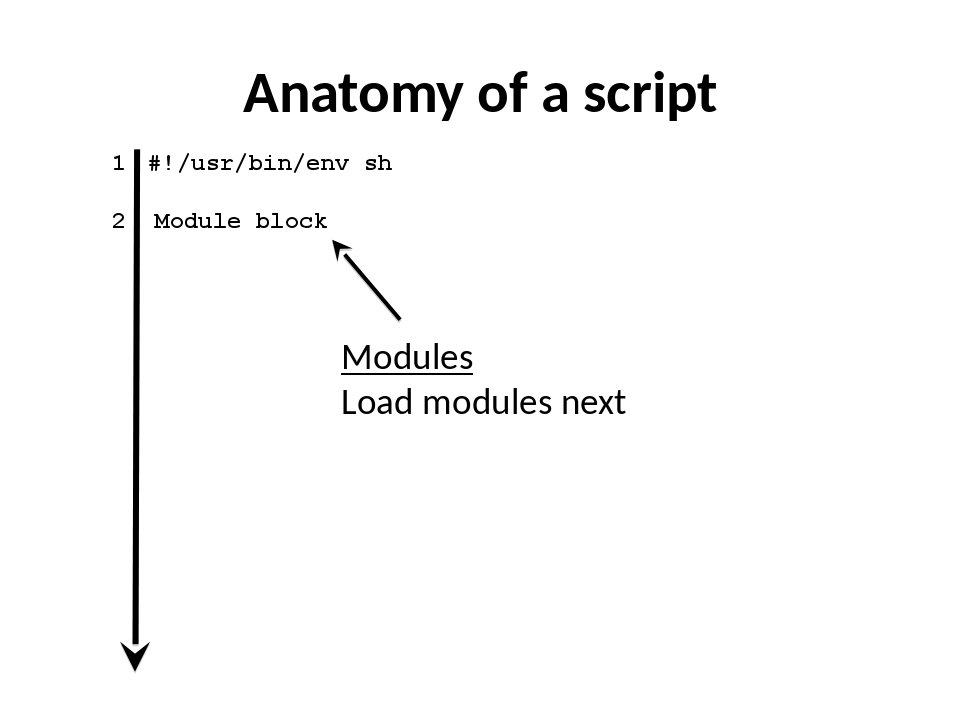
\includegraphics[width=.9\linewidth]{figures/3_anatomy_shell_script.png}
\end{frame}
\begin{frame}[label={sec:orgheadline9}]{Anatomy of a script}
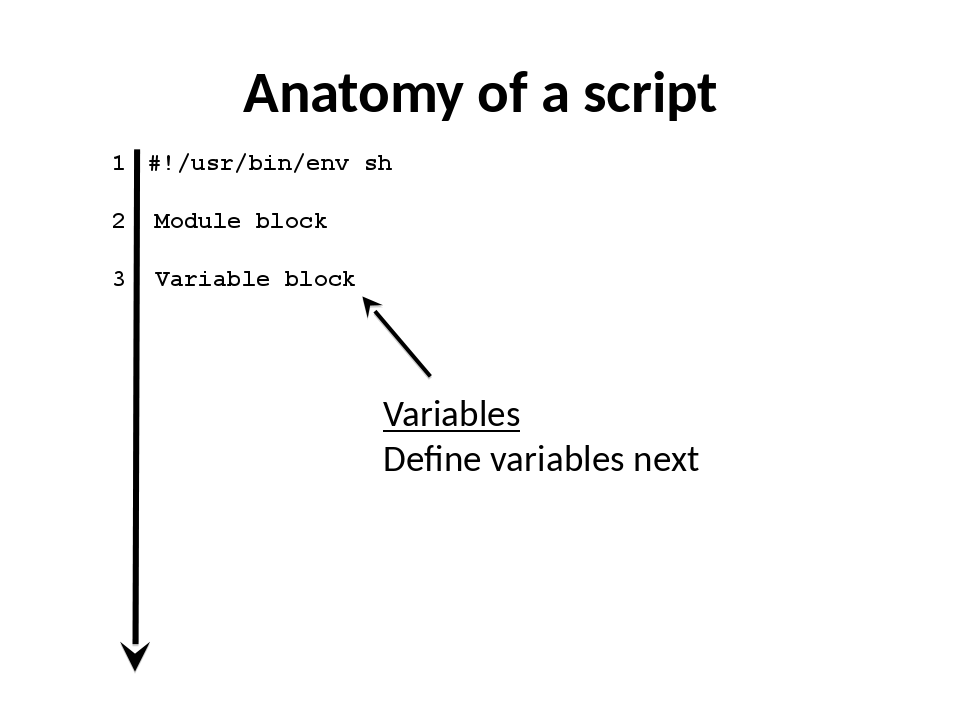
\includegraphics[width=.9\linewidth]{figures/4_anatomy_shell_script.png}
\end{frame}
\begin{frame}[label={sec:orgheadline10}]{Anatomy of a script}
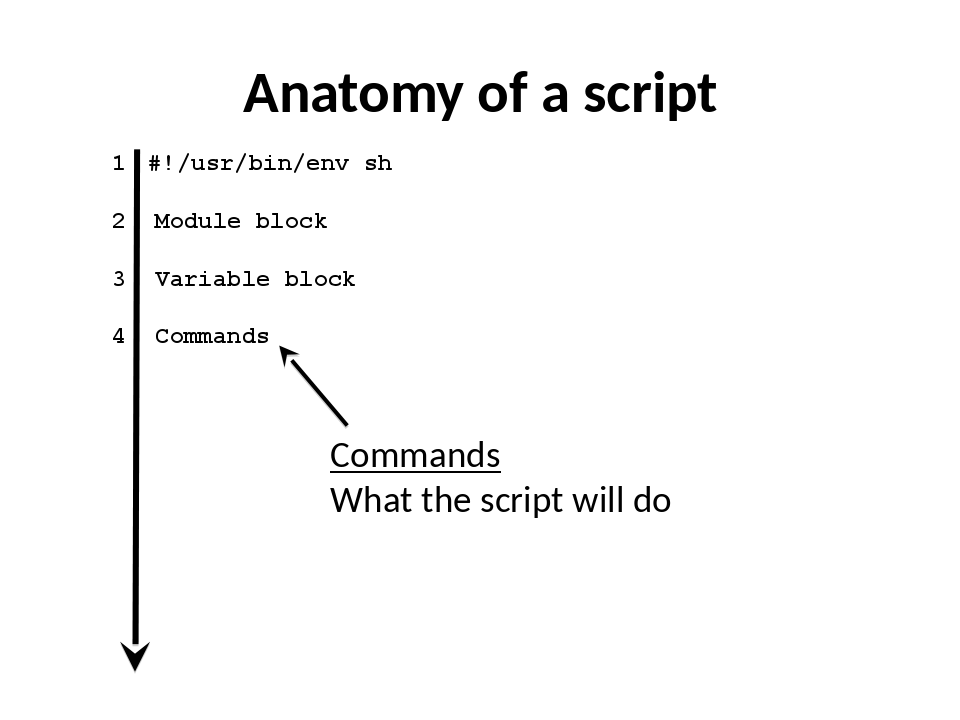
\includegraphics[width=.9\linewidth]{figures/5_anatomy_shell_script.png}
\end{frame}
\begin{frame}[label={sec:orgheadline11}]{What are variables?}
\begin{enumerate}[<+->]
\item Environmental variables
\begin{itemize}
\item used by 1 or more applications
\item \$HOME, \$PATH, \$SHELL, etc.
\end{itemize}
\item User defined variables
\begin{itemize}
\item can be anything (assume env variable names are \alert{reserved})
\item best practice
\begin{itemize}
\item indicative of what it stores
\item contains no special characters (i.e., \$)
\item separated by underscores raw\_counts
\end{itemize}
\end{itemize}
\end{enumerate}
\end{frame}
\begin{frame}[label={sec:orgheadline12}]{Why are variables important?}
\end{frame}
\begin{frame}[label={sec:orgheadline13}]{Why are variables important?}
\begin{enumerate}[<+->]
\item tidy code
\item easily readable
\item less mistakes
\begin{itemize}
\item type once use multiple times
\end{itemize}
\end{enumerate}
\end{frame}

\begin{frame}[fragile,label={sec:orgheadline14}]{Variable creation}
 \begin{enumerate}
\item directly
\end{enumerate}
\lstset{language=sh,label= ,caption= ,captionpos=b,numbers=none}
\begin{lstlisting}
wd=${HOME}/analysis_directory
echo ${wd}
\end{lstlisting}

\begin{verbatim}
/home/ssefick/analysis_directory
\end{verbatim}
\end{frame}

\begin{frame}[fragile,label={sec:orgheadline15}]{Variable creation}
 \begin{enumerate}
\item directly
\end{enumerate}
\lstset{language=sh,label= ,caption= ,captionpos=b,numbers=none}
\begin{lstlisting}
wd=${HOME}/analysis_directory
echo ${wd}
\end{lstlisting}

\begin{verbatim}
/home/ssefick/analysis_directory
\end{verbatim}

\begin{enumerate}
\item dynamically
\end{enumerate}
\lstset{language=sh,label= ,caption= ,captionpos=b,numbers=none}
\begin{lstlisting}
##direct
input_dir=input
##dynamic
files=(`ls ${input_dir} | grep sh$`)
echo ${files[@]}
\end{lstlisting}

\begin{verbatim}
awesome_script1.sh awesome_script2.sh awesome_script3.sh
\end{verbatim}
\end{frame}

\section{Bash Scripting Example}
\label{sec:orgheadline26}
\begin{frame}[label={sec:orgheadline17}]{An example: work smarter not harder}
\begin{enumerate}[<+->]
\item I accidentally named files with \alert{.sh} and not \alert{.pl}
\item What we know about the problem
\begin{itemize}
\item more than 1 mislabeled file
\item Contained in a folder called input
\end{itemize}
\item What is a sensible way to go about this?
\item Let's write a little script to fix it
\end{enumerate}
\end{frame}

\begin{frame}[label={sec:orgheadline18}]{Let's build a script interactively}
\begin{block}{Parts of a script}
\begin{enumerate}[<+->]
\item Shebang
-language specific
\item Module block
\begin{itemize}
\item all HPC modules (e.g., module load)
\end{itemize}
\item Variable block
\begin{itemize}
\item all variables
\end{itemize}
\item Commands
\begin{itemize}
\item instruction set
\end{itemize}
\end{enumerate}
\end{block}
\end{frame}

\begin{frame}[fragile,label={sec:orgheadline19}]{input}
 \begin{enumerate}
\item I think the files are in "input"
\end{enumerate}
\begin{block}{Let's check}
\lstset{language=sh,label= ,caption= ,captionpos=b,numbers=none}
\begin{lstlisting}
#########################
wd=`ls input | grep sh$`
echo ${wd}
\end{lstlisting}

\begin{verbatim}
awesome_script1.sh awesome_script2.sh awesome_script3.sh
\end{verbatim}
\end{block}
\end{frame}

\begin{frame}[fragile,label={sec:orgheadline20}]{Shebang and module block}
 \begin{block}{shebang}
\begin{enumerate}
\item top of file
\end{enumerate}
\lstset{language=sh,label= ,caption= ,captionpos=b,numbers=none}
\begin{lstlisting}
#########################
#!/usr/bin/env sh
#########################
\end{lstlisting}
\end{block}
\end{frame}

\begin{frame}[fragile,label={sec:orgheadline21}]{Shebang and module block}
 \begin{block}{shebang}
\begin{enumerate}
\item top of file
\end{enumerate}
\lstset{language=sh,label= ,caption= ,captionpos=b,numbers=none}
\begin{lstlisting}
#########################
#!/usr/bin/env sh
#########################
\end{lstlisting}
\end{block}
\begin{block}{module block}
\begin{enumerate}
\item Load all modules here
\item Easily find/remember what modules loaded
\item No modules to load because I built this presentation on a PC
\end{enumerate}
\lstset{language=sh,label= ,caption= ,captionpos=b,numbers=none}
\begin{lstlisting}
######################
##Modules
##module load something
######################
\end{lstlisting}
\end{block}
\end{frame}

\begin{frame}[fragile,label={sec:orgheadline22}]{Variable Block}
 \begin{enumerate}
\item Easily find input/output directories
\item Tidy programming
\end{enumerate}
\begin{block}{variable block}
\lstset{language=sh,label= ,caption= ,captionpos=b,numbers=none}
\begin{lstlisting}
########################
##Variables
input_dir=input
out_dir=output
##input/output files arrays
files=(`ls ${input_dir} | grep sh$`)
out_files=(`echo ${files[@]} | sed s/sh/pl/g`)

##parameter expansion
##parameter/patten/string
input_with_path=( "${files[@]/#/${input_dir}/}" )
output_with_path=( "${out_files[@]/#/${out_dir}/}" )
########################
\end{lstlisting}
\end{block}
\end{frame}

\begin{frame}[fragile,label={sec:orgheadline23}]{Commands}
 \begin{block}{For loop}
\lstset{language=sh,label= ,caption= ,captionpos=b,numbers=none}
\begin{lstlisting}
########################
##commands
##make the output dir
mkdir -p ${out_dir}

##for loop
##use length to iterate in order to index input output arrays
for ((i=0; i<${#input_with_path[@]}; i++)); do

    echo ${i}

    echo cp ${input_with_path[${i}]} ${output_with_path[${i}]} 

done
######################
\end{lstlisting}
\end{block}
\end{frame}

\begin{frame}[fragile,label={sec:orgheadline24}]{Understanding the script}
 \begin{columns}
\begin{column}{0.5\columnwidth}
\lstset{language=sh,label= ,caption= ,captionpos=b,numbers=none}
\begin{lstlisting}
files=(`ls ${input_dir} | grep sh$`)
\end{lstlisting}

\begin{center}
\begin{tabular}{l}
awesome\_script1.sh\\
awesome\_script2.sh\\
awesome\_script3.sh\\
\end{tabular}
\end{center}

\lstset{language=sh,label= ,caption= ,captionpos=b,numbers=none}
\begin{lstlisting}
out_files=(`echo ${files[@]} | sed s/sh/pl/g`)
\end{lstlisting}

\begin{center}
\begin{tabular}{l}
awesome\_script1.pl\\
awesome\_script2.pl\\
awesome\_script3.pl\\
\end{tabular}
\end{center}
\end{column}

\begin{column}{0.5\columnwidth}
\lstset{language=sh,label= ,caption= ,captionpos=b,numbers=none}
\begin{lstlisting}
input_with_path=( "${files[@]/#/${input_dir}/}" )
\end{lstlisting}

\begin{center}
\begin{tabular}{l}
input/awesome\_script1.sh\\
input/awesome\_script2.sh\\
input/awesome\_script3.sh\\
\end{tabular}
\end{center}

\lstset{language=sh,label= ,caption= ,captionpos=b,numbers=none}
\begin{lstlisting}
output_with_path=( "${out_files[@]/#/${out_dir}/}" )
\end{lstlisting}

\begin{center}
\begin{tabular}{l}
output/awesome\_script1.pl\\
output/awesome\_script2.pl\\
output/awesome\_script3.pl\\
\end{tabular}
\end{center}
\end{column}
\end{columns}
\end{frame}

\begin{frame}[fragile,label={sec:orgheadline25}]{Understanding the for loop}
 \lstset{language=sh,label= ,caption= ,captionpos=b,numbers=none}
\begin{lstlisting}
for ((i=0; i<${#input_with_path[@]}; i++)); do

    ${i}

    cp ${input_with_path[${i}]} ${output_with_path[${i}]} 

done
\end{lstlisting}

\lstset{language=sh,label= ,caption= ,captionpos=b,numbers=none}
\begin{lstlisting}
echo ${i}
\end{lstlisting}

\begin{center}
\begin{tabular}{r}
0\\
1\\
2\\
\end{tabular}
\end{center}

\lstset{language=sh,label= ,caption= ,captionpos=b,numbers=none}
\begin{lstlisting}
cp ${input_with_path[${i}]} ${output_with_path[${i}]}
\end{lstlisting}

\begin{center}
\begin{tabular}{lll}
cp & input/awesome\_script1.sh & output/awesome\_script1.pl\\
cp & input/awesome\_script2.sh & output/awesome\_script2.pl\\
cp & input/awesome\_script3.sh & output/awesome\_script3.pl\\
\end{tabular}
\end{center}
\end{frame}

\section{Exercise}
\label{sec:orgheadline28}
\begin{frame}[label={sec:orgheadline27}]{History to script}
\begin{enumerate}[<+->]
\item blast history to script from last class
\item Use some information from today
\item Why in the world would we want to redo an analysis?
\begin{itemize}
\item reproducible research artifact
\end{itemize}
\item \textasciitilde{}20 min
\begin{itemize}
\item HW5
\end{itemize}
\end{enumerate}
\end{frame}
\section{Reproducible Research}
\label{sec:orgheadline32}
\begin{frame}[label={sec:orgheadline29}]{Gold standard: literate programming}
\textbf{\Large "Let us change our traditional attitude to the construction of programs: Instead of imagining that our main task is to instruct a computer what to do, let us concentrate rather on explaining to human beings what we want a computer to do."} -Knuth
\end{frame}
\begin{frame}[label={sec:orgheadline30}]{Some Tools}

\includegraphics[width=.9\linewidth]{figures/out.png}
\end{frame}
\begin{frame}[label={sec:orgheadline31}]{10 suggestions from the paper}
\begin{enumerate}
\item For every result, keep track of how it was produced
\item Avoid manual data manipulation steps
\item Archive the exact versions of all external programs used
\item Version control all custom scripts
\item Record all intermediate results, when possible in standardized formats
\item For analyses that include randomness, note underlying random seeds
\item Always store raw data behind plots
\item Generate hierarchical analysis output, allowing layers of increasing detail to be inspected
\item Connect textual statements to underlying results
\item Provide public access to scripts, runs, and results
\end{enumerate}
\end{frame}
\end{document}
